\documentclass[a4paper,12pt,openany]{book}

\usepackage{ZeroSeven}
\usepackage{ltablex}
\usepackage[official]{eurosym}
\usepackage[utf8]{inputenc}
\usepackage{blindtext}
\usepackage{makecell}
\usepackage{hyperref}
\titlepage{}

\author{Stefano Zanatta}
\date{2018-12-24}
\intestazioni{
\includegraphics[scale=0.3]{images/logo_intestazione}}
\pagestyle{myfront}
\begin{document}
\begin{titlepage}
	\centering
	{\huge\bfseries MegAlexa\par}
	Arricchitore di skill di Amazon Alexa
	\line(1,0){350} \\
	{\scshape\LARGE Piano di Qualifica \par}
	\vspace{1cm}
	{\scshape Gruppo ZeroSeven \par}
	\logo
	%devono essere compilati questi campi ogni volta
	\begin{tabular}{c|c}
		{\hfill \textbf{Versione}} 			& 2.0.0				\\
		{\hfill\textbf{Data Redazione}} 	& 2018-12-24	\\ 
		{\hfill\textbf{Redazione}} 			&  Stefano Zanatta \\&Andrea Deidda\\&Bianca Andreea Ciuche\\
	{\hfill\textbf{Verifica}} 				&  	Matteo Depascale\\ &Mirko Franco\\ &Andrea Deidda\\
		{\hfill\textbf{Approvazione}} 		&  			Gian Marco Bratzu\\ 
	{\hfill\textbf{Uso}} 					& 		Esterno		\\ 
	{\hfill\textbf{Distribuzione}} 			& 			Prof. Tullio Vardanega \\ & Prof. Riccardo Cardin \\ & Gruppo ZeroSeven		\\ & Zero12 s.r.l. \\
		{\hfill\textbf{Email di contatto}} & zerosevenswe@gmail.com \\
	\end{tabular}
\end{titlepage}
	

	
	\label{LastFrontPage}
	\newpage	
	\begin{center}
	\textbf{Registro delle modifiche}
	\end{center}
	\begin{center}
		\begin{tabularx}{\textwidth}{|c|c|X|X|c|}
			\hline
			\textbf{Versione} & \textbf{Data} & \textbf{Descrizione} & \textbf{Autore} & \textbf{Ruolo} \\ 
			\hline
			3.0.0 & 2019-04-11 & Approvazione per il rilascio RQ & Ludovico Brocca & Responsabile \\
			\hline
			2.1.0 & 2019-04-09 & Verifica documento & Ludovico Brocca & Verificatore \\
			\hline
			2.0.6 & 2019-04-08 & Aggiunto riferimento metriche alla sezione \S\ref{MetricheObbiettivi} &Matteo depascale & Amministratore \\
			\hline 
			2.0.5 & 2019-04-08 & Modifica sezioni \S\ref{Verifica}  e \S\ref{Validazione} & Matteo depascale & Amministratore \\
			\hline
			2.0.4 & 2019-04-08 & Aggiunti comandi personalizzati alla sezione \S\ref{NormeRedazionali} &Matteo depascale & Amministratore \\
			\hline
			2.0.3 & 2019-04-04 & Aggiunta voci a \S\ref{ListaControllo} & Matteo depascale & Amministratore \\
			\hline
			2.0.2 & 2019-04-01 & Stesura sezioni \S\ref{DiagrammiDelleClassi}, \S\ref{DiagrammiPackage}, \S\ref{DiagrammiSequenza} e \S\ref{DiagrammiAttivita}  & Bianca Andreea Ciuche & Amministratore \\
			\hline
			2.0.1 & 2019-03-23 & Modifica \ref{Documentazione fornita} Corretti numeri di sezione & Bianca Andreea Ciuche & Amministratore \\
			\hline
			2.0.0 &2019-03-07 & Approvazione per il rilascio & Gian Marco Bratzu& Responsabile\\
			\hline
			1.2.0 &2019-03-02 & Verifica documento &Andrea Deidda& Verificatore\\
			\hline
			1.1.2 &2019-02-13 &Stesura \S\ref{calcoloOre} &Ludovico Brocca& Amministratore\\
			\hline
			1.1.1 &2019-02-13 &Modifica\S \ref{anDinamica} &Ludovico Brocca& Amministratore\\
			\hline
			1.1.0 &2019-02-07 &Verifica \S\ref{processo}, \ref{metriche}, \S\ref{progettazione} &Gian Marco Bratzu& Verificatore\\
			\hline
			1.0.4 &2019-02-04&Stesura \S\ref{processo}&Ludovico Brocca& Analista\\
			\hline
			1.0.3 & 2019-02-03 & Modifica \S\ref{metriche} & Stefano Zanatta & Amministratore\\
			\hline
			1.0.2 & 2019-02-02 & Stesura \S\ref{metriche} & Bianca Andreea Ciuche & Amministratore\\
			\hline
			1.0.1 & 2018-01-12 & Stesura \S\ref{progettazione} & Mirko Franco & Amministratore \\
			\hline
			1.0.0 & 2018-01-09 & Approvazione per il rilascio & Stefano Zanatta & Responsabile\\
			\hline
			0.2.0 & 2018-12-29 & Verifica documento & Stefano Zanatta & Verificatore\\
			\hline
			0.1.0 & 2018-12-18 & Verifica \S\ref{PdS} & Mirko Franco & Verificatore\\
			\hline
			0.0.6 & 2018-12-21 & Modifica \S\ref{Intro} & Andrea Deidda & Amministratore\\
			\hline
			0.0.5 & 2018-12-17 & Stesura \S\ref{Po} & Ludovico Brocca & Amministratore\\
			\hline
			0.0.4 & 2018-12-16 & Stesura \S\ref{Pp} & Matteo Depascale & Amministratore\\
			\hline
			0.0.3 & 2018-12-16 & Stesura \S\ref{Intro} & Bianca Ciuche & Amministratore\\
			\hline
			0.0.2 & 2018-12-10 & Stesura \S\ref{PdS} & Gian Marco Bratzu & Amministratore\\	
			\hline
			0.0.1 & 2018-12-08 & Struttura documento  & Ludovico Brocca & Amministratore\\
			\hline
	\end{tabularx}
	\end{center}

\newpage
	\pagestyle{mymain}
	\tableofcontents
	\listoftables
	\chapter{Introduzione}
\label{introduzione}
\section{Scopo del documento}
Il \textit{Piano di Qualifica} ha lo scopo di definire gli obbiettivi di qualità che il gruppo perseguita per il proprio prodotto. Per ottenere tali obbiettivi è necessario un processo di verifica continua di ogni attività. Questo consente di rilevare e correggere le anomalie riscontrate tempestivamente.\\
Questo documento descrive nel dettaglio la qualità dei processi più vicini nel tempo e ad alto livello quelli più lontani, per poi essere aggiornato con nuovi contenuti ogni volta che il gruppo lo ritiene necessario.
\section{Scopo del prodotto}
Lo scopo del progetto è quello di sviluppare un applicativo Mobile in grado di creare delle routine personalizzate per gli utenti gestibili tramite\glossario{Alexa}di\glossario{Amazon}. L'obbiettivo è quello di creare\glossario{skill}in grado di avviare\glossario{workflow}creati dagli utenti fornendogli dei\glossario{connettori}.
\section{Glossario}
Al fine di evitare ogni ambiguità di linguaggio e massimizzare la comprensione dei documenti, i termini tecnici, di dominio, gli acronimi e le parole che necessitano di essere chiarite, sono riportate nel \textit{Glossario v1.0.0}.\\
Ogni occorrenza di vocaboli presenti nel \textit{Glossario} è marcata da una "G" maiuscola in pedice.
\section{Riferimenti}
\subsection{Normativi}
\begin{itemize}
	\item  \textbf{Norme di Progetto}: \textit{Norme di Progetto v1.0.0};
	\item \textbf{Capitolato$_{G}$ C4}:\glossario{MegAlexa}: arricchitore di skill di Amazon Alexa.
	\item \textbf{Ciclo di Deming}
	\footnote{\url{https://it.wikipedia.org/wiki/Ciclo_di_Deming}}
\end{itemize}
\subsection{Informativi}\label{rfinf}
\begin{itemize}
	\item \textbf{Piano di Progetto}: \textit{Piano di Progetto v1.0.0};
	\item \textbf{Complessità ciclomatica}
	\item \textbf{Software Testing Fundamentals: Methods and Metrics} di Marnie L. Hutcheson, Wiley Publishing, Inc.  
	\footnote{\url{https://www.math.unipd.it/~tullio/IS-1/2018/Progetto/C4.pdf}}.
	
	
\end{itemize}

	\chapter{Qualità di Processo}
\label{processo} 
\section{Scopo}
Al fine di garantire la massima efficacia del prodotto finale è necessario controllare e misurare i processi che concorrono alla sua realizzazione; a tal fine si fa riferimento ai principi stabiliti dallo standard ISO/IEC 12207 per la suddivisione dei processi in moduli disaccoppiati ma comunque coesi fra loro e alle responsabilità derivanti da ciascuno di essi.
Viene applicato inoltre il ciclo di Deming (PDCA), al fine di assicurare un miglioramento continuo delle attività di processo. 

\section{Processi}

\subsection{Pianificazione}
Per misurare l'efficacia della pianificazione vengono adottate le seguenti metriche 

\subsubsection{BCWP: Budgeted Cost Of Work Performed}\label{bcwp}
Utilizzato per il calcolo di Cost Variance e Schedule Variance, rappresenta (in giorni) il valore delle attività svolte.
\begin{itemize}
	\item Range accettazione: [>= 0];
	\item Range ottimale: [>= 0].
\end{itemize}
\subsubsection{BCWS: Budgeted Cost of Work Scheduled}\label{bcws}
Rappresenta il costo in giorni preventivato per il processo in esame (è detto anche Planned Value):
\begin{itemize}
\item Range accettazione: [>=0].
\item Range ottimale: [>= 0].
\end{itemize}

\subsubsection{ACWP: Actual Cost of Work Performed}\label{acwp}
Rappresenta il costo (in \euro) effettivamente sostenuto al momento del calcolo:
\begin{itemize}
	\item Range accettazione: [>=0].
	\item Range ottimale: [>= 0].
\end{itemize}

\subsubsection{SV: Schedule Variance}
Metrica che indica se si è in anticipo o in ritardo rispetto alla schedulazione delle attività di progetto.
Essa è il risultato della seguente formula:\\
\begin{center}
	
	$SV = $\hyperref[bcwp]{BCWP} $-$\hyperref[bcws]{BCWS}
	
\end{center}

\begin{itemize}
	\item Range accettazione: $-BCWS *10\%$;
	\item Range ottimale: [>= 0].
\end{itemize}



\subsection{Miglioramento}
%todo
%STANDARD SPICE??%
\subsection{Costo}
Per verificare che i costi siano conformi a quanto preventivato nel \textit{Piano di Progetto}, ciascun processo viene misurato tramite la sua \textbf{Cost Variance(CV)}, un valore positivo indica il rispetto dei costi preventivati, essa viene calcolata nel seguente modo:\\ 

\begin{center}
	\begin{math}
	CV = BCWP - ACWP
	\end{math}
\end{center}
\begin{itemize}
	\item[] \textbf{ACWP} (Actual Cost of Work Performed) rappresenta il costo(in giorni) effettivamente sostenuto al momento del calcolo. 
\end{itemize}
Dove: BCWP e ACWP sono descritte rispettivamente nelle sezioni \ref{bcwp} e \ref{acwp}.

\begin{itemize}
	\item Range accettazione: Viene accettato uno scostamento massimo del 10\% rispetto ai costi preventivati;
	\item Range ottimale: [>= 0].
\end{itemize}


\subsection{Analisi dei rischi}
%todo
%spice +sv
\section{Metriche}
tabella-metriche
	\chapter{Qualità di Prodotto}
\label{prodotto}
\section{Scopo}
Per riuscire a garantire una buona qualità di prodotto, sono state individuate nello standard ISO/IEC 25010 le principali caratteristiche che i prodotti devono avere definendone le sotto-caratteristiche che le compongono e individuandone delle metriche adeguate per poter misurare ogni aspetto.

\section{Qualità documento}
\label{documento}
Il team si impegna a produrre dei documenti di alta qualità, rispettando le seguenti caratteristiche.
\subsection{Ortografia}
\subsubsection{Obbiettivi}
Un documento, per essere privo di errori grammaticali e ortografici, viene controllato su diversi ambienti: durante la redazione, tramite il controllo automatico integrato nell'ambiente di lavoro; nel repository condiviso, tramite il correttore automatico eseguito da Travis-ci (con notifica in caso di errori); durante la verifica, da parte di un\glossario{Verificatore}.\\
Le metriche utilizzate per la valutazione, definite nelle Norme di Progetto in Appendice B, sono le seguenti:
\begin{itemize}
	\item MPR001 numero di errori ortografici.
\end{itemize}
\subsection{Comprensibilità e leggibilità}
\subsubsection{Obbiettivi}
Per misurare la leggibilità di un documento il gruppo ha scelto di utilizzare l'indice di\glossario{Gulpease}. Questo viene calcolato automaticamente ogni volta che il documento viene modificato nel repository condiviso.\\
Le metriche utilizzate per la valutazione, definite nelle Norme di Progetto in Appendice B, sono le seguenti:
\begin{itemize}
	\item MPR002 indice di Gulpease$_{G}$.
\end{itemize}
\subsection{Correttezza dei contenuti}
\subsubsection{Obbiettivi}
La correttezza del documento è data anche dalla coerenza dei contenuti. Ogni membro del gruppo deve redigere dei buoni documenti, i verificatori devono controllarli e seguire le procedure definite nelle \textit{Norme di Progetto v2.0.0}.\\
Le metriche utilizzate per la valutazione, definite nelle Norme di Progetto in Appendice B, sono le seguenti:
\begin{itemize}
	\item MPR003 Numero di errori inerenti alla correttezza dei documenti.
\end{itemize}
\subsection{Adesione alla norme interne}
\subsubsection{Obbiettivi}
I documenti devono rispettare le Norme di Progetto. I \glossario{Verificatori} hanno il compito di avvisare il \textit{Responsabile} come definito nelle \textit{Norme di Progetto v2.0.0}.\\
Le metriche utilizzate per la valutazione, definite nelle Norme di Progetto in Appendice B, sono le seguenti:
\begin{itemize}
	\item MPR004 numero di errori inerenti alle Norme di Progetto.
\end{itemize}

\section{Qualità del software}
\label{software}

\subsection{Funzionalità}
Rappresenta la capacità del prodotto software di provvedere le funzionalità necessarie a soddisfare i requisiti individuati nel documento Analisi dei Requisiti v2.0.0. 
\subsubsection{Obbiettivi }Il prodotto dovrà possedere le seguenti caratteristiche:
\begin{itemize}
	\item \textbf{Efficacia funzionale:} Indice che determina il grado di copertura dei requisiti;
	\item \textbf{Correttezza:} Indice che determina la correttezza dei risultati forniti dal software.
\end{itemize}

Le metriche utilizzate per la valutazione, definite nelle Norme di Progetto in Appendice B, sono le seguenti:
\begin{itemize}
	\item MPR005 Completezza dell'implementazione funzionale;
	\item MPR006 Correttezza rispetto alle attese.
\end{itemize}

\subsection{Affidabilità}
Rappresenta la capacità del prodotto software di svolgere correttamente le sue funzionalità mantenendo delle buone prestazioni al verificarsi di situazioni anomale.

\subsubsection{Obbiettivi} Il prodotto dovrà possedere le seguenti caratteristiche :
\begin{itemize}
	\item \textbf{Tolleranza agli errori:} Il\glossario{prodotto}software continua a lavorare correttamente in presenza di errori dovuti a uno scorretto uso dell'applicativo;
	\item \textbf{Recuperabilità:} Nel caso in cui si presenta un'anomalia, l'applicativo è in grado di recuperare i dati e ripristinare lo stato interrotto.
\end{itemize}

Le metriche utilizzate per la valutazione, definite nelle Norme di Progetto in Appendice B, sono le seguenti:
\begin{itemize}
	\item MPR007 Totalità di failure.
\end{itemize}


\subsection{Efficienza}
Rappresenta la capacità di un prodotto software di realizzare le funzioni richieste nel minor tempo possibile e con l'uso del minimo numero di risorse necessarie. 
\subsubsection{Obbiettivi } Il prodotto dovrà possedere le seguenti caratteristiche :
\begin{itemize}
	\item \textbf{Comportamento rispetto al tempo:} per svolgere le  funzioni richieste il prodotto software deve fornire adeguati tempi di risposta ed elaborazione;
	\item \textbf{Utilizzo delle risorse:} il software nello svolgimento delle funzionalità deve utilizzare un appropriato numero e tipo di risorse.
\end{itemize}
Le metriche utilizzate per la valutazione, definite nelle Norme di Progetto in Appendice B, sono le seguenti:
\begin{itemize}
	\item MPR008 Tempo di risposta.
\end{itemize}

\subsection{Usabilità}
L'usabilità rappresenta il grado di facilità e soddisfazione con cui si compie l'interazione tra l'uomo e il \textit{prodotto$_{G}$}, ovvero l'efficacia, l'efficienza e la soddisfazione con le quali gli utenti raggiungono determinati obbiettivi in determinati contesti.
\subsubsection{Obbiettivi } Il prodotto dovrà possedere le seguenti caratteristiche:
\begin{itemize}
	\item \textbf{Apprendibilità:} livello di facilità con cui il prodotto può essere appreso dagli utenti per portare a termine determinati obiettivi con efficacia, efficienza, sicurezza e soddisfazione;
	\item \textbf{Comprensibilità:} livello a cui gli utenti riescono a riconoscere se il prodotto è adeguato per i loro bisogni;
	\item \textbf{Protezione dall'errore:} Rappresenta il grado con cui il\glossario{prodotto}protegge l'utente dal commettere errori;
	\item \textbf{Estetica dell'interfaccia utente:} livello a cui un'interfaccia utente risulta piacevole per l'utente che la utilizza;
	\item \textbf{Accessibilità:} Si intende la possibilità di fornire i servizi anche a coloro che sono affetti da disabilità temporanee e non, che quindi utilizzano tecnologie ausiliarie.
	Nel caso dell'echo alcune disabilità sono per ora vincolanti in quanto presuppongono necessariamente l'utilizzo della voce.
\end{itemize}
Le metriche utilizzate per la valutazione, definite nelle Norme di Progetto in Appendice B, sono le seguenti:
\begin{itemize}
	\item MPR009 Comprensibilità delle funzioni offerte;
	\item MPR010 Facilità di apprendimento.
\end{itemize}

\subsection{Manutenibilità}
Rappresenta la capacità del\glossario{prodotto}di essere modificato tramite correzioni, miglioramenti e adattamenti.
\subsubsection{Obbiettivi } Il prodotto dovrà possedere le seguenti caratteristiche :
\begin{itemize}
	\item \textbf{Analizzabilità:} Il software deve poter essere analizzato per poter trovare gli errori;
	\item \textbf{Modificabilità:} Il prodotto deve permettere la modifica delle sue parti;
	\item \textbf{Modularità:} Il prodotto è diviso in parti che svolgono compiti ben precisi;
	\item \textbf{Riusabilità:} Le parti del software possono essere riusate in altre applicazioni;
	\item \textbf{Testabilità:} Il software deve essere testabile per consentire la validazione e l'approvazione di modifiche.
\end{itemize}	Le metriche utilizzate per la valutazione, definite nelle Norme di Progetto in Appendice B, sono le seguenti:
\begin{itemize}
	\item MPR011 Capacità di analisi failure;
	\item MPR012 Impatto delle modifiche.
\end{itemize}

\section{Tabella delle metriche}
\label{Tab3.1}
\begin{center}
	\begin{tabularx}\textwidth{|c|X|X|X|}
		\hline 
		\textbf{ID} & \textbf{Nome} & \textbf{Range di accettazione}  & \textbf{Range di ottimalità}  \\ 
		\hline
		\multicolumn{4}{|c|}{\textbf{Qualità documento}} \\
		\hline
		MPR001 & Numero di errori ortografici & 0\% & 0\%\\
		\hline
		MPR002 & Indice di Gulpease & 40-100 & 50-100 \\
		\hline
		MPR003 & Numero di errori inerenti alla correttezza
		dei documenti &80-100 &90-100 \\
		\hline
		MPR004 & Numero di errori inerenti alle Norme di Progetto & 85-100 & 90-100 \\
		\hline
		\multicolumn{4}{|c|}{\textbf{Qualità software}} \\
		\hline
		MPR005 & Completezza dell'implementazione funzionale & 100\% & 100\%\\
		\hline
		MPR006 & Correttezza rispetto alle attese & 90\%-100\%  & 100\% \\
		\hline
		MPR007 & Totalità di failure & 0\%-10\% & 0\% \\
		\hline
		MPR008 & Tempo di risposta & 0-8 sec & 0-3 sec \\
		\hline
		MPR009 & Comprensibilità delle funzioni offerte & 75\%-100\% &90\%-100\% \\
		\hline
		MPR010 & Facilità di apprendimento &0-20 min & 0-10 min\\
		\hline
		MPR011 & Capacità di analisi failure & 60\% -100 \%& 80\%-100\%\\
		\hline
		MPR012 & Impatto delle modifiche & 0\%-20\%&0\%-15\% \\
		\hline
		\caption{Tabella delle metriche del prodotto}
	\end{tabularx}
\end{center}

	\begin{appendices}
		\chapter{Specifica test}
\label{test}
\section{Test di Sistema}
\normalsize
\begin{longtable}{|c|>{}m{8cm}|c|}
\hline 
\textbf{Id test} & \textbf{Descrizione} & \textbf{Stato}\\
\hline
\endhead
\hypertarget{TSFO2}{TSFO2} & Il gruppo esegue l'applicazione e controlla che il login funziona correttamente. & \textit{Non Implementato}\\ \hline
\hypertarget{TSFO15}{TSFO15} & Eseguire l'applicazione, creare un nuovo \textit{workflow$_{G}$}, aggiunge dei blocchi a piacere e salvare il workflow. Bisogna verificare che il workflow sia presente nel database. & \textit{Non Implementato}\\ \hline
\hypertarget{TSFO16}{TSFO16} & Avviare l'applicazione ed eliminare un workflow. & \textit{Non Implementato}\\ \hline
\hypertarget{TSFO17.1}{TSFO17.1} & Avviare l'applicazione e modificare il nome di un workflow, poi verificare che sia stato effettivamente modificato nel database. & \textit{Non Implementato}\\ \hline
\hypertarget{TSFO17.2}{TSFO17.2} & Il test consiste nell' eseguire l'applicazione e modificare un workflow aggiungendo un blocco, modificandone un altro ed eliminandone un terzo. In seguito verificare che il database sia stato effettivamente modificato. & \textit{Non Implementato}\\ \hline
\caption[Test di Sistema]{Test di sistema}
\label{tabella:test1}
\end{longtable}
\clearpage
\subsection{Tracciamento test di sistema-requisiti}
Ogni test di sistema viene eseguito per validare un requisito, definito nell'\analisideirequisiti.
\normalsize
\begin{longtable}{|>{\centering}m{5cm}|m{5cm}<{\centering}|}
\hline
\textbf{Test} & \textbf{Requisito}\\
\hline
\endhead
\hyperlink{TSFO2}{TSFO2} & RFO2\\ \hline
\hyperlink{TSFO15}{TSFO15} & RFO15\\ \hline
\hyperlink{TSFO16}{TSFO16} & RFO16\\ \hline
\hyperlink{TSFO17.1}{TSFO17.1} & RFO17.1\\ \hline
\hyperlink{TSFO17.2}{TSFO17.2} & RFO17.2\\ \hline
\caption[Tracciamento test di sistema-requisiti]{Tracciamento test di sistema-requisiti}
\label{tabella:ts-requi}
\end{longtable}

\section{Test di integrazione}
\normalsize
\begin{longtable}{|c|>{}m{8cm}|c|}
\hline 
\textbf{Id test} & \textbf{Descrizione} & \textbf{Stato}\\
\hline
\endhead
\hypertarget{TI1}{TI1} & Viene testata l'applicazione Android ad ogni sua modifica nel repository \textit{Github$_{G}$}, attraverso \textit{Travis CI$_{G}$}. L'applicazione deve compilare e non produrre warning. & \textit{Non Implementato}\\ \hline
\hypertarget{TI2}{TI2} & La skill\glossario{Android}è soggetta a integrazione continua, attraverso Travis-CI. & \textit{Non Implementato}\\ \hline
\hypertarget{TI3}{TI3} & La skill viene pubblicata in automatico (ad ogni modifica nel repository) in Aws Lambda e viene eseguito un test per controllare che funzioni. Questo test non assicura il funzionamento della skill, quindi è necessario un controllo umano (più controlli sono richiesti in caso di un numero alto di commit nel repository). & \textit{Non Implementato}\\ \hline
\hypertarget{TI4}{TI4} & Ad ogni commit nel repository, Travis-CI controlla che il collegamento tra la Skill e AWS \textit{API}\glossario{Gateway}funzioni. Questo viene fatto attraverso una semplice chiamata post a una funzione MOCK (per ridurre il traffico a\glossario{DynamoDB}e alle Lambda). & \textit{Non Implementato}\\ \hline
\hypertarget{TI5}{TI5} & Controllare che il collegamento tra API Gateway, Lambda e DynamoDB funzioni, eseguendo dei test automatici appositi. Questa operazione deve essere eseguita poco frequentemente, in quanto potrebbe aumentare i costi dei servizi \textit{AWS$_{G}$}. & \textit{Non Implementato}\\ \hline
\caption[Test di Integrazione]{Test di integrazione}
\label{tabella:test2}
\end{longtable}

\subsection{Tracciamento test di integrazione-componenti}
Nella seguente tabella viene riportato il tracciamento tra test di Integrazione e Package, definiti in \normediprogetto.
\normalsize
\begin{longtable}{|>{\centering}m{3cm}|m{9cm}<{\centering}|}
\hline
\textbf{Test} & \textbf{Componente}\\
\hline
\endhead
\hyperlink{TI1}{TI1} & \texttt{megalexa}\\ \hline
\hyperlink{TI2}{TI2} & {\texttt{MegAlexaSkill}}\\ \hline
\hyperlink{TI3}{TI3} & {\texttt{MegAlexaSkill::lambda}}\\ \hline
\hyperlink{TI4}{TI4} & {\texttt{MegAlexaSkill::lambda::connection}}\\ \hline
\hyperlink{TI5}{TI5} & {\texttt{megalexa::adapters}}\\ \hline
\caption[Tracciamento test di integrazione-componenti]{Tracciamento test di integrazione-componenti}
\label{tabella:ts-requi}
\end{longtable}

\section{Test di unità}
Questa sezione verrà compilata durante il periodo di progettazione di dettaglio e codifica, per applicare il \textit{Test Driven Development$_{G}$} (come richiesto dalla proponente).
		\chapter{Resoconto delle attività di verifica}
\label{resoconto}
\section{Analisi}
Nel periodo antecedente la Revisione dei Requisiti sono stati verificati i documenti ed i processi applicando quanto descritto nelle \textit{Norme di Progetto v2.0.0}.\\
L'analisi statica è stata effettuata secondo i criteri e le modalità indicate nelle \textit{Norme di Progetto}.\\ 
Per gli errori riscontrati effettuando \textit{walkthrough$_{G}$}, si è provveduto a correggere le anomalie riscontrate e sono stati riportati nella lista di controllo nelle \textit{Norme di Progetto v2.0.0} per permettere di effettuare inspection successivamente.\\
L'\textit{inspection$_{G}$} viene effettuata utilizzando la lista di controllo precedentemente stilata. \\
Si sono poi calcolate le metriche descritte nelle \textit{Norme di Progetto}.\\
L'avanzamento dei processi viene poi valutato secondo le metriche descritte nelle \textit{Norme di Progetto}. 
\subsection{Verifica dei processi}
Per il\glossario{processo}di stesura dei documenti, il calcolo delle metriche di Budget Variance e di Schedule Variance è stato effettuato sul valore complessivo delle ore impiegate dal totale dei componenti del gruppo.\\
Per le successive fasi del \textit{progetto$_{G}$}, il gruppo si propone di automatizzare il processo di calcolo delle ore impiegate, con il dettaglio puntuale dei singoli processi.
Lo Schedule Variance totale è di -1 ore e il Budget Variance totale equivale a -25\euro.
\begin{comment}
\begin{tabularx}{\textwidth}{|C|C|C|}
	\hline
	\textbf{Macro-Attività}& \textbf{SV}&\textbf{BV}\\
	\hline
	\textit{Norme di Progetto}    & \euro & \euro\\
	\textit{Piano di Progetto}    & \euro & \euro\\
	\textit{Studio di Fattibilità} & \euro & \euro\\
	\textit{Analisi dei Requisiti}& \euro & \euro\\
	\textit{Piano di Qualifica}   & \euro & \euro\\
	\textit{Glossario}            & \euro & \euro\\
	\hline
	\caption{Esito verifica processi}
\end{tabularx}
\end{comment}
\\
\subsection{Verifica dei documenti}
\begin{tabularx}{\textwidth}{|C|c|C|}
	\hline
	\textbf{Documento}& \textbf{Indice di Gulpease}&\textbf{Esito}\\
	\hline
	\endhead
	\textit{Norme di Progetto}    & 76 & Superato \\
	\textit{Piano di Progetto}    & 64 & Superato \\
	\textit{Studio di Fattibilità} & 61 & Superato\\
	\textit{Analisi dei Requisiti}& 80 & Superato \\
	\textit{Piano di Qualifica}   & 67 & Superato \\
	\textit{Glossario}            & 68 & Superato \\
	\hline
	\caption{Esito della verifica documenti}
\end{tabularx}

\section{Revisione Analisi}
\label{revisione}
Durante il breve periodo di Revisione Analisi, il gruppo si è preparato allo sviluppo del POC e ha apportato delle correzione ai documenti, migliorando i propri processi. 
\subsection{Verifica dei processi}
I miglioramenti principali (tutti descritti nelle \textit{Norme di Progetto v2.0.0}) sono stati:
\begin{itemize}
	\item Automatizzato il calcolo delle ore di lavoro integrando \glossario{Harvest} ad \glossario{Asana};
	\item Automatizzato il calcolo dell'indice di Gulpease, tramite script;
	\item Se dei documenti contenenti degli errori grammaticali raggiungono la repository, un bot avvisa per email chi ha commesso l'errore e invia una notifica al gruppo.
\end{itemize}

\subsubsection{MP001 Schedule variance}
\begin{figure} [h]
    \centering
	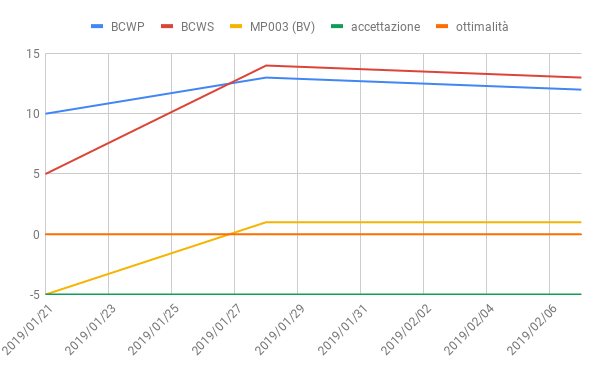
\includegraphics[scale=0.5]{./images/svRa.png}
	\caption{\textit{MP001 - Revisione Analisi}}\label{}
\end{figure}
\pagebreak
\subsubsection{MP002 Budget variance}
\begin{figure} [h]
    \centering
	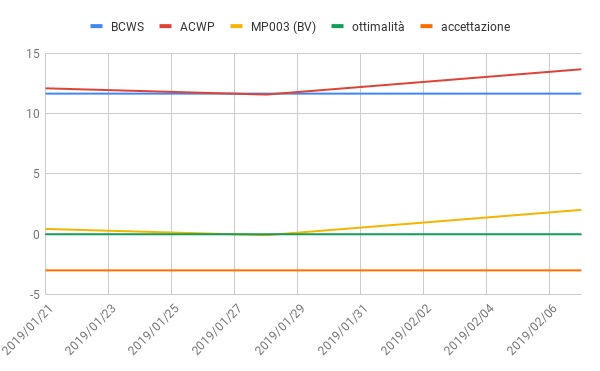
\includegraphics[scale=0.5]{./images/bvra.png}
	\caption{\textit{MP002 - Revisione Analisi}}\label{}
\end{figure}

\section{Progettazione della base tecnologica}
\label{progettazione}
\subsection{MP001: Schedule variance}
\begin{figure} [h]
    \centering
	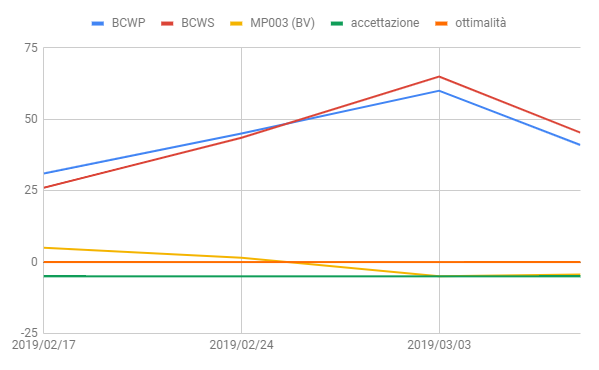
\includegraphics[scale=0.5]{./images/svP.png}
	\caption{\textit{MP001 - Progettazione della base tecnologica}}\label{}
\end{figure}
\pagebreak
\subsection{MP002: Budget variance}
\begin{figure} [h]
    \centering
	\includegraphics[scale=0.5]{./images/bvP.png}
	\caption{\textit{MP002 - Progettazione della base tecnologica}}\label{}
\end{figure}

\subsection{MP003: SPICE capability level}
Di seguito vengono riportati i livelli di maturità raggiunti dai processi eseguiti durante lo sviluppo del \glossario{poc}. Data l'inesperienza, non viene raggiunto il livello di accettazione richiesto (3) per la maggior parte dei processi, ma il gruppo sta lavorando per migliorare.
\begin{figure} [h]
    \centering
	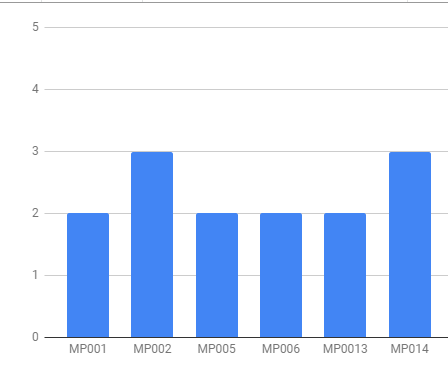
\includegraphics[scale=0.5]{./images/15504.png}
    \caption{\textit{MP003 - ISO/IEC 15504 }}\label{}
\end{figure}

\subsection{MP005:  Occorrenza rischi non previsti}
\textbf{rischi non previsti: 2}
\begin{itemize}
	\item Un aggiornamento automatico di \glossario{Android Studio} ha completamente rimosso una libreria utilizzata dall'applicazione mobile, quindi il gruppo ha perso tempo per implementane una alternativa. Questo è successo perché la libreria in questione era deprecata. Per evitare problemi simili, l'utilizzo di librerie deprecate è stato vietato, come descritto nelle \textit{Norme di Progetto};
	\item E' stata inserita una chiave di accesso Amazon nel repository. Il gruppo è stato avvisato da Amazon, e ha dovuto creare nuove chiavi per tutti i membri.
\end{itemize}

\subsection{MP006: Indisponibilità dei servizi}
\textbf{indisponibilità dei servizi: 0}\\
Durante il periodo di progettazione della base tecnologica, il gruppo non ha riscontrato problemi riguardanti il downtime di servizi esterni.

\subsection{MP013: Percentuale build superate}
Viene fatta distinzione tra Android e Skill, in quanto vengono contenute in repository diversi.\\
Le build non superate sono 24 su 134 per la Skill e 29 su 232 per Android. Entrambe superano il range di ottimalità (80\%);
\begin{figure} [h]
    \centering
	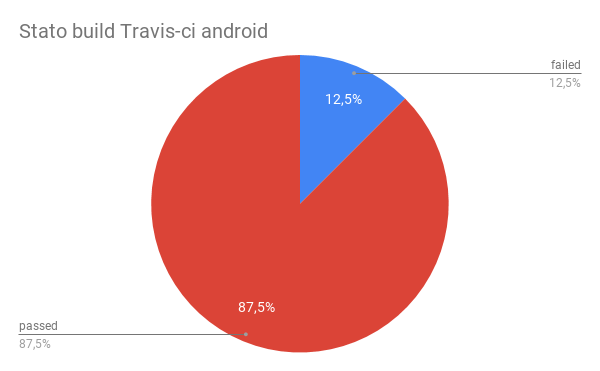
\includegraphics[scale=0.5]{./images/StatobuildTravis-ciandroid.png}
    \caption{\textit{MP013 - Android - Progettazione della base tecnologica}}\label{}
\end{figure}\\
\begin{figure} [h]
    \centering
	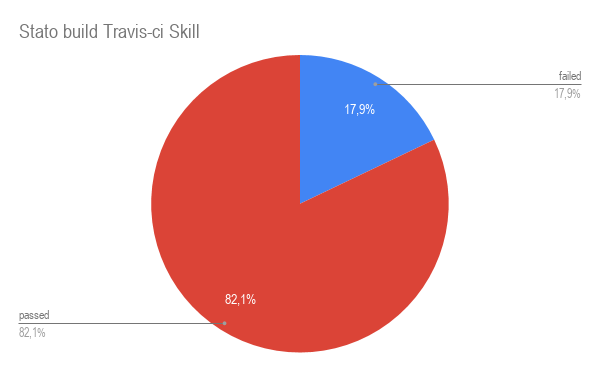
\includegraphics[scale=0.5]{./images/StatobuildTravis-ciSkill.png}
    \caption{\textit{MP013 - Skill - Progettazione della base tecnologica}}\label{}
\end{figure}
\clearpage

\subsection{MP014: Media commit giornaliera}
Come si può vedere dai grafici, il numero di commit è stato abbastanza costante, con un aumento del carico di lavoro durante la fine di febbraio.
\begin{figure} [h]
    \centering
	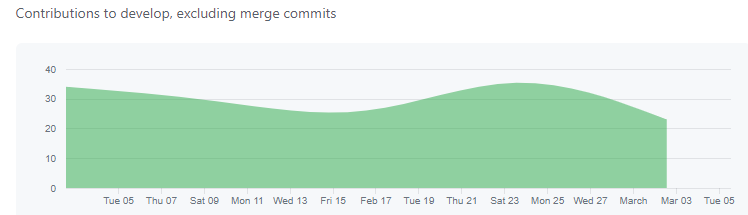
\includegraphics[scale=0.5]{./images/dailycommits_kotlin.PNG}
    \caption{\textit{MP014 - Android- Progettazione della base tecnologica}}\label{}
\end{figure}
\begin{figure} [h]
    \centering
	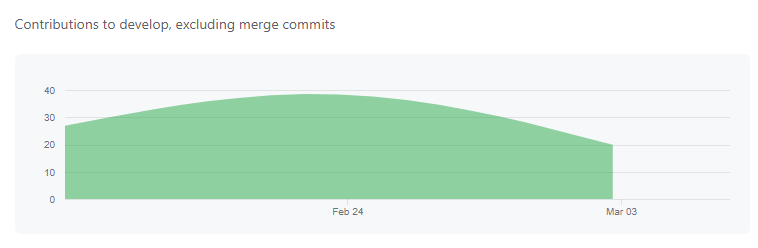
\includegraphics[scale=0.5]{./images/daycommits_js.PNG}
    \caption{\textit{MP014 - Skill - Progettazione della base tecnologica}}\label{}
\end{figure}

\subsection{MP015, MP016: Percentuale requisiti soddisfatti}
\begin{figure} [h]
    \centering
	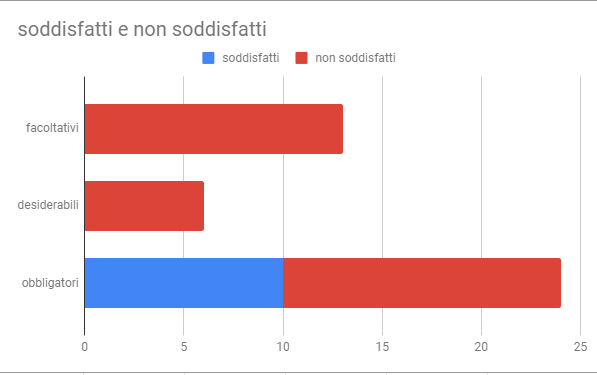
\includegraphics[scale=0.5]{./images/req.PNG}
    \caption{\textit{MP015 - MP016 Tipologia di requisiti}}\label{}
\end{figure}
\begin{figure} [h]
    \centering
	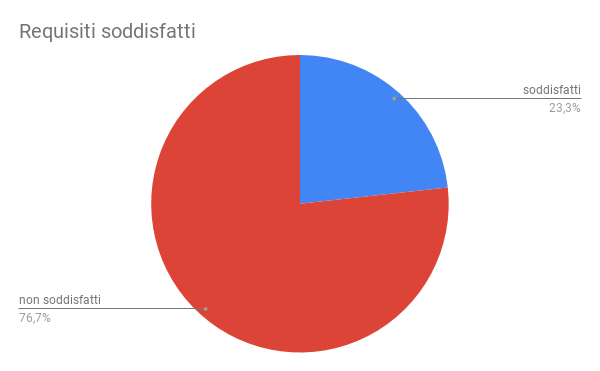
\includegraphics[scale=0.5]{./images/RequisitiSoddisfatti.png}
    \caption{\textit{MP015 - MP015 Differenza soddisfatti e non soddisfatti}}\label{}
\end{figure}

\newpage
\section{Progettazione di dettaglio e codifica}
Questa sezione verrà compilata alla fine del periodo di Progettazione della base tecnologica.
\section{Verifica e collaudo}
Questa sezione verrà compilata alla fine del periodo di Verifica e collaudo.
	\end{appendices}

			
	\label{LastPage}

\end{document}
